% 
% file: projectWriteup.tex 
% author: Ian Woods
%
 
\documentclass[11pt]{article}
\usepackage{amsmath}
\usepackage{graphicx}
%\usepackage{indentfirst}
%\setlength{\evensidemargin}{0in}
%\setlength{\textheight}{9in}
%\setlength{\textwidth}{6.5in}
\setlength{\topmargin}{-0.5in}

% Sample macros -- how you define new commands
% My own set of frequently-used macros have grown to many hundreds of lines.
% Here are some simple samples.
\newcommand{\Adv}{{\mathbf{Adv}}}       
\newcommand{\prp}{{\mathrm{prp}}}                  % How to define new commands 
\newcommand{\calK}{{\cal K}}
\newcommand{\outputs}{{\Rightarrow}}                
\newcommand{\getsr}{{\:\stackrel{{\scriptscriptstyle\hspace{0.2em}\$}}{\leftarrow}\:}}
\newcommand{\andthen}{{\::\;\;}}    % \, \: \; for thinspace, medspace, thickspace
\newcommand{\Rand}[1]{{\mathrm{Rand}[{#1}]}}       % A command with one argument
\newcommand{\Perm}[1]{{\mathrm{Perm}[{#1}]}}       
\newcommand{\Randd}[2]{{\mathrm{Rand}[{#1},{#2}]}} % and with two arguments


%%%%%%%%%%%%%%%%%%%%%%%%%%%%%%%%%%%%%%%%%%%%%%%%%%%%%%%%%%%%%%%%%%%%%%%%%%%
\title{\bf ECS 171 - Forest Cover Project Write-up: Pine Subgroup\\[2ex] }
\date{\today}
\author{\bf Ian Woods, Jesse Dyer, Miguel Covarrubias}

\begin{document}
\maketitle


%%%%%%%%%%%%%%%%%%%%%%%%%%%%%%%%%%%%%%%%%%%%%%%%%%%%%%%%
\section*{Brief Description of KNN} 
The $k$-Nearest Neighbors (KNN) Algorithm involves classifying a given sample as a particular type, given the type of the $k$ closest samples to it, as determined by some distance function. Our initial approach was to use a standard Euclidean distance function, defined as follows:
\\
$\sqrt{\sum\limits_{k = 1}^n (x_{jk} - x_{ik})^2}$
\\
We decided to begin with this naive approach to isolate failure points (essentially, if something were to work incorrectly, we could rule out the distance function as failure point).
We debated creating a distance function tailored to the dataset by hand, or by simply trying many different possible distance functions. However, we decided to generate a distance function with the largest-margin nearest neighbors algorithm (more precisely, we generated a transformation matrix that was used to transform the data, and still used the Euclidean distance).
\\
Using different values for $k$ can theoretically alter the predicted results - for example, if a sample of unknown type is closest to a sample of type $A$ with a calculated distance of 1, but two samples of type $B$ are at a distance of 1.1 from our unknown sample, choosing $k$ = 1 will yield the result $A$ for the unknown's type, and $k$ = 3 will yield the result $B$. We decided to test a wide range of $k$ values.
\section*{Results of Standard KNN Algorithm for Various K Values}
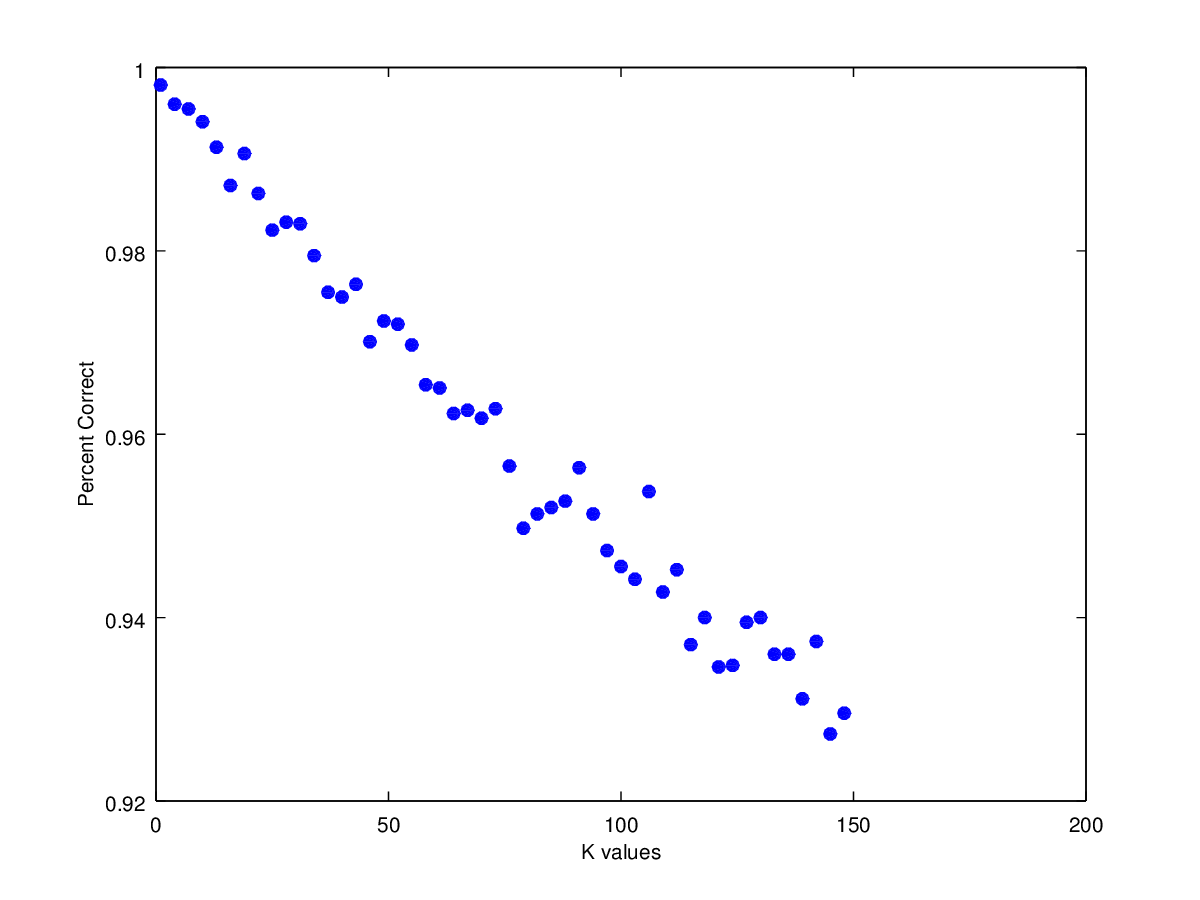
\includegraphics[scale=.75]{kValuesGraph.png}
\\
As can be seen in the above graph, increasing the value of $k$ reduced the accuracy of the classifier. We tested over a range from 1 to 150 with a step size of 3 (to reduce computation time while still revealing the overall trend). This makes intuitive sense - imagine a KNN implementation with $k = $ the size of the data set. Say there are $n$ samples of the most common type, and $z$ total samples. Every sample would be labeled as the most common sample, resulting in an accuracy of $\frac{n}{z}$.
\section*{Brief Description of LMNN}
LMNN (Largest Margin Nearest Neighbors) is a variant of KNN that can be implemented in two ways. One method is to learn a Mahalanobis distance function, which measures the distance (in standard deviations) from the center of a cluster of similarly typed samples. Another method, and the method our implementation used, is to learn a transformation matrix that, when applied to the dataset, yields higher correct classification rates. It learns this matrix by iteratively applying small perturbations to the transformation matrix with the goal of maintaining a large distance between "impostors" (close neighbors that are of the wrong type) and the perimeters that surround groups of similarly-typed neighbors. LMNN is very helpful because it saves use the trouble of testing many different distance functions, or trying to derive a distance function by hand for each particular dataset. Pictured below are the results of our LMNN classifier, compared to the standard KNN classifier.
\section*{Results of LMNN}
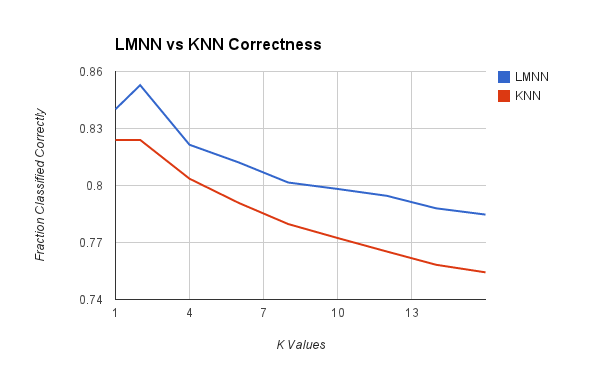
\includegraphics[scale=.75]{knnvslmnn.png}

LMNN was able to boost the correct classification percentage in every case. On average, we saw 2.46\% better classification rates. It took quite a lot of extra time to learn the distance function, though - running the LMNN algorithm on the entire UCI dataset took on the order of one hour on a relatively high-powered desktop computer (quad core Intel i5 processor at 3.4GHz, all CPUs at 95\% + load for most of the computation).
\\
Below are the ROC and PR curves for our LMNN classifier for each of the 7 forest cover types.
\includegraphics[scale=.5]{Aspen.jpg}

\end{document}




%
%
%
%We ran 20 preliminary trial runs on the standard KNN algorithm and found that, at these %low values, the predictor is relatively stable as $k$ changes. I THINK THIS IS NO LONGER %CORRECT
%
%\begin{center}
%  \begin{tabular}{ l | c | c | c | c | c | c | c | c | c | c | c | c | c | c | c | c | c %| c | c | r }
%    \hline
%    $k$ & 1 & 2 & 3 & 4 & 5 & 6 & 7 & 8 \\ \hline
%    \% correct & 0.909845 & 0.908847 & 0.910052 & 0.908158 & 0.908503 & 0.910465 & %0.915628 & 0.910981 \\
%    \hline
%  \end{tabular}
%\end{center}
%
%\begin{flushleft}
%  \begin{tabular}{ l | c | c | c | c | c | c | c | c | c | c | c | c | c | c | c | c | c %| c | c | r }
%    \hline
%    $k$ & 9 & 10 & 11 & 12 & 13 & 14 & 15 & 16 \\ \hline
%    \% correct & 0.913150 &  0.909122 & 0.908124 & 0.907504 & 0.906816 & 0.910843 & %0.911979 &  0.906506 \\
%    \hline
%  \end{tabular}
%\end{flushleft}


%Note to whoever is reading this before it's submitted - We will test higher $k$ values %against the entire dataset (these were tested against 1/10th of the dataset to save %time). 
%Additionally, we will put up some pretty graphs, etc.
